\documentclass[12pt,a4paper]{report}
\usepackage[utf8]{inputenc}
\usepackage{amsmath}
\usepackage{amsfonts}
\usepackage{amssymb}
\usepackage{makeidx}
\usepackage{graphicx}
\usepackage{cancel}
\usepackage{geometry}
\usepackage[ngerman]{babel}
\geometry{a4paper, top=20mm, left=10mm, right=10mm, bottom=20mm}
\author{Marius Ketterer}
\title{Praktikum Regelungstechnik 2 Abgabe Versuch 1 Digitale Übertragungsglieder}
\begin{document}

\maketitle
\tableofcontents

\chapter{Tiefpass 1.Ordnung}
\section{Aufstellen der Übertragungsfunktionen im s-Bereich inklusive Halteglied}
Aufstellen der Übertagungsfunktionen
\begin{equation}
G_{PT1}(s) = \frac{K}{1+Ts} 
\end{equation}
\begin{equation}
H(s) = \frac{1-e^{-T_As}}{s}
\end{equation}

Aus der Reihenschaltung von $H(s)$ und $G_{PT1}(s)$ ergibt $G(s) = H(s)*G_{PT1}(s)$\\
\section{Transformation in den z-Bereich über Korrespondenztabelle}
Will man diese Übertragungsfunktion nun in den z-Bereich transformieren geht man folgendermaßen vor.
\begin{equation}
G(z) = \mathcal{Z}\{\mathcal{L}^{-1}\{H(s)*G_{PT1}(s)\}\}|_{kT_A}
\end{equation}

Nun wird $H(s)$ eingesetzt:
\begin{equation}
G(z)=
\mathcal{Z}\left\{\mathcal{L}^{-1}\left\{\frac{(1-e^{-T_As})* G_{PT1}(s)}{s}\right\}\right\}|_{kT_A}
= \mathcal{Z}\left\{\mathcal{L}^{-1}\left\{\frac{G_{PT1}(s)}{s}\right\}\right\}
-\mathcal{Z}\left\{\mathcal{L}^{-1}\left\{\frac{G_{PT1}(s)}{s}*e^{-T_As}\right\}\right\}|_{kT_A}
\end{equation}

Eine Multiplikation mit $e^{-T_As}$ bedeutet eine Rechtsverschiebung um $T_A$ was im im z-Bereich eine Multiplikation mit $z^{-1}$ entspricht.
\begin{equation}
G(z) = \mathcal{Z}\left\{(1-e^{-T_As})*\frac{G_{PT1}(s)}{s}\right\} = (1-z^{-1})*\mathcal{Z}\left\{\frac{G_{PT1}(s)}{s}\right\}
\end{equation}

Somit lässt sich generell sagen, dass die z-Transformierte Übertragungsfunktion einer Reihenschaltung eines Übertragungsgliedes $G(s)$ und eines Haltegliedes, sich folgendermaßen berechnen lässt.
\begin{equation}
G(z) = (1-z^{-1})*\mathcal{Z}\left\{\frac{G(s)}{s}\right\}
\label{generell}
\end{equation}


Setzt man nun auch $G_{PT1}(s)$ ein erhält man folgendes
\begin{equation}
G(z) = (1-z^{-1})*\mathcal{Z}\left\{\frac{K}{s(1+Ts)}\right\} =  (1-z^{-1})*\mathcal{Z}\left\{K\frac{\frac{1}{T}}{s(\frac{1}{T}+s)}\right\}
\end{equation}

Transformieren mit Hilfe der Korrespondenzentabelle(Nr.8)
\begin{equation}
G(z) = K*\cancel{(1-z^{-1})}*
\frac{(1-e^{-\frac{T_A}{T}})z^{-1}}
{\cancel{(1-z^{-1})}(1-e^{-\frac{T_A}{T}}z^{-1})}
\end{equation}
Daraus ergibt sich: 
\begin{equation}
G(z) = \frac{K*z^{-1}-K*e^{-\frac{T_A}{T}}z^{-1}}
{1-e^{-\frac{T_A}{T}}z^{-1}} 
\end{equation}
Einsetzen der Werte
\begin{equation}
K = 3; T = 4; T_A = 0,5s
\end{equation}
\begin{equation}
G(z) = \frac{3z^{-1}-3*e^{-\frac{0,5}{4}}z^{-1}}
{1-e^{-\frac{0,5}{4}}z^{-1}} = \frac{0,352z^{-1}}{1-0,882z^{-1}} = \frac{Y}{X}
\end{equation}
\begin{equation}
Y- 0,882z^{-1}Y = 0,352z^{-1}X
\end{equation}
Nach $ Y $ aufgelöst ergibt das:
\begin{equation}
\Rightarrow Y = 0,352z^{-1}X + 0,882z^{-1}Y
\end{equation}
\section{Darstellung als Strukturplan}
\begin{figure}[ht]
	\centering
	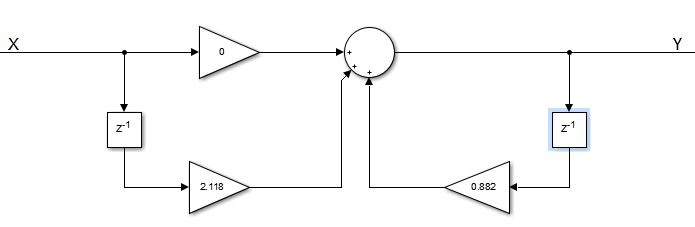
\includegraphics[width=0.8\linewidth]{marius/PT1}
	\caption{Struckturplan PT1}
	\label{fig:PT1}
\end{figure}

\section{Simulationsergebnisse}
\begin{figure}[ht]
	\centering
	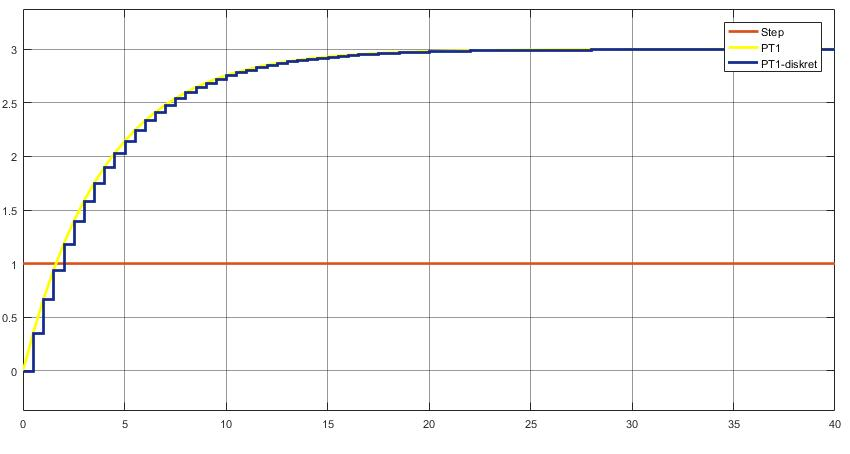
\includegraphics[width=0.9\linewidth]{marius/PT1_Step}
	\caption{Sprungantwort des diskreten PT1-Filter}
	\label{fig:PT1_Step}
\end{figure}
\begin{figure}[ht]
\centering
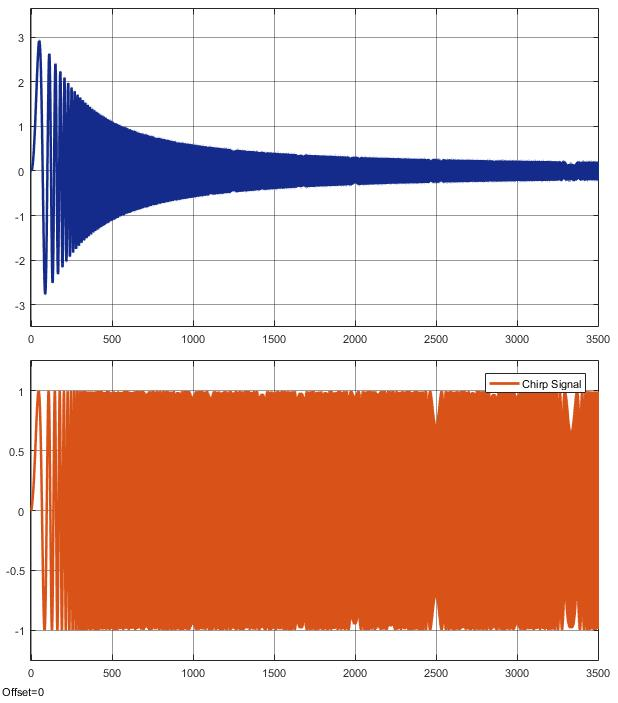
\includegraphics[width=0.9\linewidth]{marius/PT1_Chirp_0,0001-1Hz}
\caption{Chirpsignal auf den diskreten PT1-Filter}
\label{fig:PT1_Chirp}
\end{figure}




\chapter{Hochpass 1. Ordnung}
\section{Aufstellen der Übertragungsfunktionen im s-Bereich inklusive Halteglied}
Aufstellen der Übertagungsfunktionen

\begin{equation}
G_{DT1}(s) = \frac{Ks}{1+Ts} 
\end{equation}
Transformieren in den Z-Bereich. Dazu wird die Formel \ref{generell} angewendet
\begin{equation}
G(z) = (1-z^{-1})*\mathcal{Z}\left\{\frac{G_{DT1}(s)}{s}\right\} = (1-z^{-1})*\mathcal{Z}\left\{\frac{K\cancel{s}}{\cancel{s}(1+Ts)}\right\} = (1-z^{-1})*\mathcal{Z}\left\{\frac{K}{(1+Ts)}\right\}
\end{equation}

\begin{equation}
G(z) = (1-z^{-1})*\mathcal{Z}\left\{\frac{K}{T}\frac{1}{s+\frac{1}{T}}\right\}
\end{equation}
\section{Transformation in den z-Bereich über Korrespondenztabelle}
Transformieren mit Hilfe der Korrespondenzentabelle(Nr.4)
\begin{equation}
G(z) = \frac{K}{T}*(1-z^{-1})*
\frac{1}
{1-e^{-\frac{T_A}{T}}z^{-1}}
\end{equation}
Daraus ergibt sich: 
\begin{equation}
G(z) = \frac{K-K*z^{-1}}
{T-e^{-\frac{T_A}{T}}z^{-1}*T} 
\end{equation}
Einsetzen der Werte
\begin{equation}
K = 3; T = 4; T_A = 0,5s
\end{equation}
\begin{equation}
G(z) = \frac{3-3*z^{-1}}
{4-e^{-\frac{0,5}{4}}z^{-1}*4} = \frac{3-3*z^{-1}}
{4-3,53z^{-1}} = \frac{Y}{X}
\end{equation}
\begin{equation}
4Y- 3,53z^{-1}Y = 3X -3z^{-1}X
\end{equation}
Nach $ Y $ aufgelöst ergibt das:
\begin{equation}
4Y = 3X- 3z^{-1}X + 3,53z^{-1}Y
\end{equation}
\begin{equation}
\Rightarrow Y = \frac{3}{4}X- \frac{3}{4}z^{-1}X + 0,8825z^{-1}Y
\end{equation}
\section{Darstellung als Strukturplan}
\begin{figure}[ht]
	\centering
	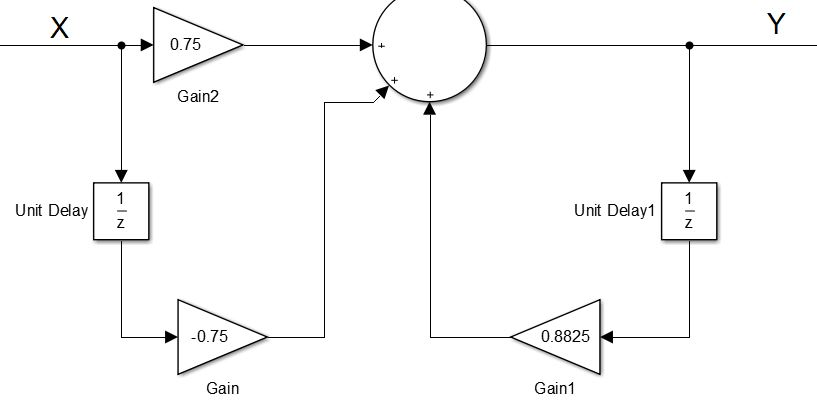
\includegraphics[width=0.8\linewidth]{marius/DT1}
	\caption{Struckturplan DT1}
	\label{fig:DT1}
\end{figure}


\section{Simulationsergebnisse}
\begin{figure}[ht]
	\centering
	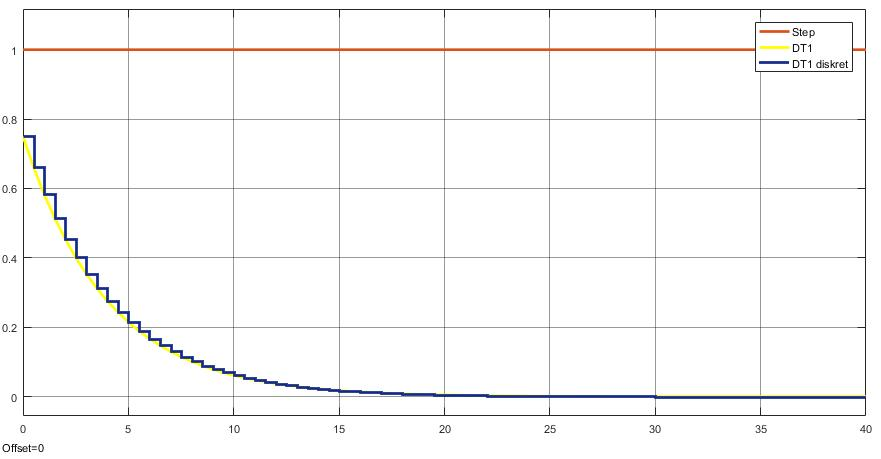
\includegraphics[width=0.9\linewidth]{marius/DT1_Step}
	\caption{Sprungantwort des diskreten DT1-Filter}
	\label{fig:DT1_Step}
\end{figure}
\begin{figure}[ht]
	\centering
	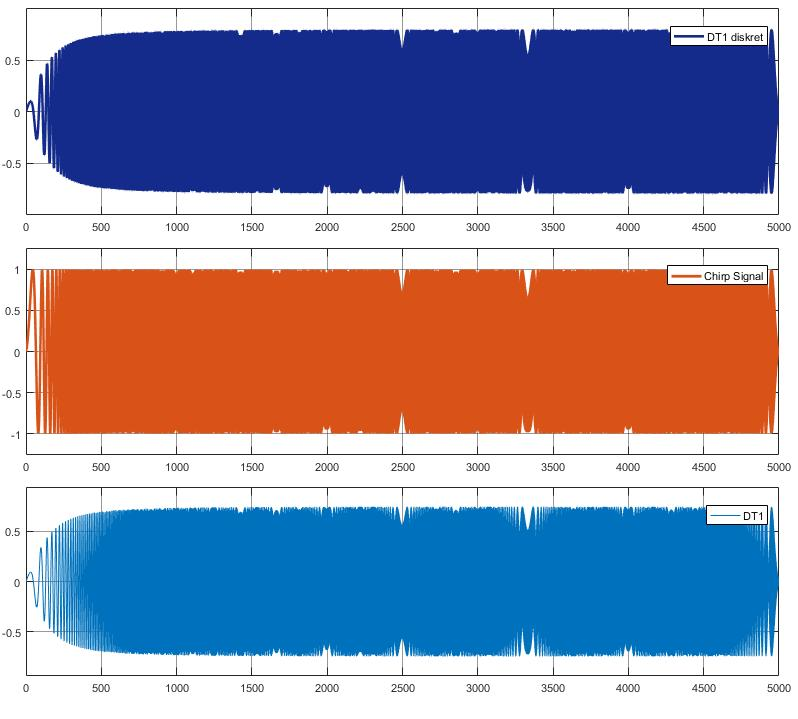
\includegraphics[width=0.9\linewidth]{marius/DT1_Chrip_0,001-0,2Hz}
	\caption{Chirpsignal auf den diskreten DT1-Filter}
	\label{fig:DT1_Chirp}
\end{figure}

\chapter{PID-Regler}
\begin{equation}
G_{PID}(s) = K_P*\left( 1+ \frac{1}{T_Ns} + T_Vs \right)
\end{equation}

\begin{equation}
y(t) = K_R \left[e(t) +\frac{1}{T_N}\int e(t) dt+ t_V \frac{de(t)}{dt}\right]
\end{equation}

\begin{equation}
y_k = K_R \left[e_k +\frac{1}{T_N}\sum_{i=0}^{k-1}e_iT_A+ T_V \frac{e_k-e_{k-1}}{T_A}\right]
\end{equation}

Nun wird $y_{k-1}$ berechnet:
\begin{equation}
y_{k-1} = K_R \left[e_{k-1} +\frac{1}{T_N}\sum_{i=0}^{k-2}e_iT_A+ T_V \frac{e_{k-1}-e_{k-2}}{T_A}\right]
\end{equation}

Die Differenz aus den beiden ergibt:
\begin{equation}
y_k-y_{k-1} = K_R \left[e_k-e_{k-1} 
+\frac{T_A}{T_N}e_{k-1}
+ \frac{T_V}{T_A}(e_k-2e_{k-1}+e_{k-2})\right]
\end{equation}

\begin{equation}
y_k = y_{k-1}+ K_R \left[
\left(1+\frac{T_V}{T_A}\right)e_k 
-\left(1-\frac{T_A}{T_N}+2\frac{T_V}{T_A}\right)e_{k-1}
+ \frac{T_V}{T_A}e_{k-2}
\right]
\end{equation}

Daraus ergeben sich folgenende Koeffizienten:
\begin{equation}
a_1 = 1, b_0 = K_R\left(1+\frac{T_V}{T_A}\right),
b_1 = -K_R \left(1-\frac{T_A}{T_N}+2\frac{T_V}{T_A}\right),
b_2 = K_R \frac{T_V}{T_A}
\end{equation}

Nun hat man die Übertragungsfunktion:

\begin{equation}
G(z)= \frac{b_0*z^2+b_1*z+b_2}{z^2-a_1*z} = \frac{b_0+b_1*z^{-1}+b_2*z^{-2}}{1-a_1*z^{-1}} = \frac{Y}{X}
\end{equation}

\begin{equation}
	(b_0+b_1*z^{-1}+b_2*z^{-2})*X= Y-a_1*z^{-1}Y
\end{equation}
Nach Y aufgelöst
\begin{equation}
Y= 	(b_0+b_1*z^{-1}+b_2*z^{-2})*X + a_1*z^{-1}Y
\end{equation}
Nun werden in die Werte $K=3; T_N=4; T_V= 1 $ und $T_A = 0,5$ in die Koeffizientengleichungen eingesetzt. Man erhält:
\begin{equation}
b_0 = 9; b_1 = -14,625; b_2= 6
\end{equation} Diese werden nun in die Gleichung eingesetzt und der Struckturplan erstellt.\\


\section{Darstellung als Strukturplan}

\begin{figure}[h]
	\centering
	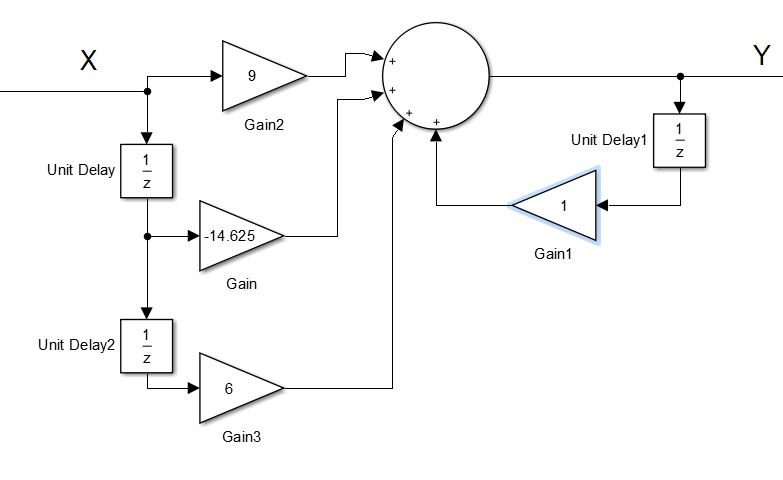
\includegraphics[width=0.8\linewidth]{marius/PID}
	\caption{Struckturplan PID}
	\label{fig:PID}
\end{figure}

\section{Simulationsergebnisse}
\begin{figure}[ht]
	\centering
	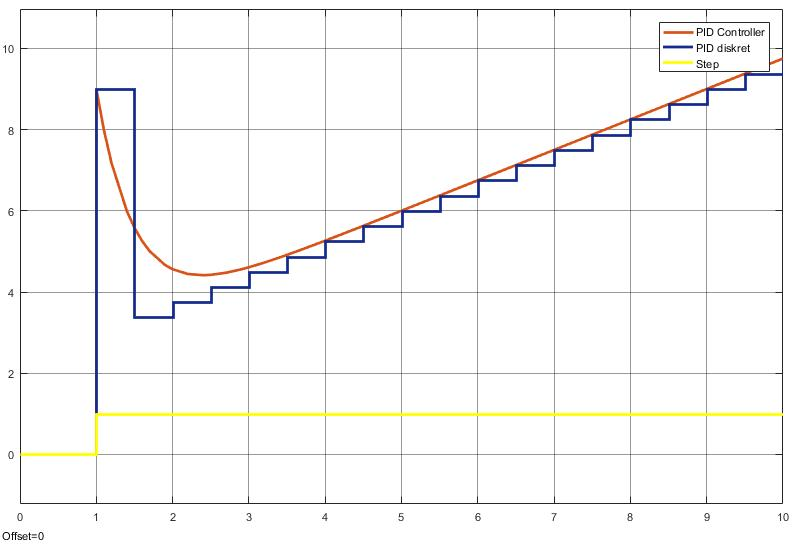
\includegraphics[width=0.9\linewidth]{marius/PID_Step}
	\caption{Sprungantwort des diskreten PID-Reglers}
	\label{fig:PID_Step}
\end{figure}
\begin{figure}[ht]
	\centering
	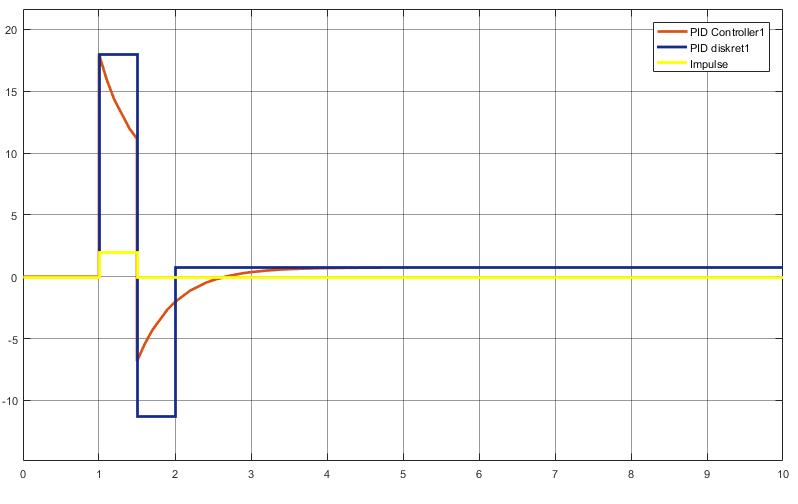
\includegraphics[width=0.9\linewidth]{marius/PID_Impulse}
	\caption{Impulseantwort des diskreten PID-Reglers}
	\label{fig:PID_Impulse}
\end{figure}

\chapter{Gleitender Mittelwertbilder(FIR)}

\begin{equation}
Y = \frac{1}{4}X*(1+z^{-1}+z^{-2}+z^{-3})
\end{equation}

\section{Darstellung als Strukturplan}
\begin{figure}[ht]
	\centering
	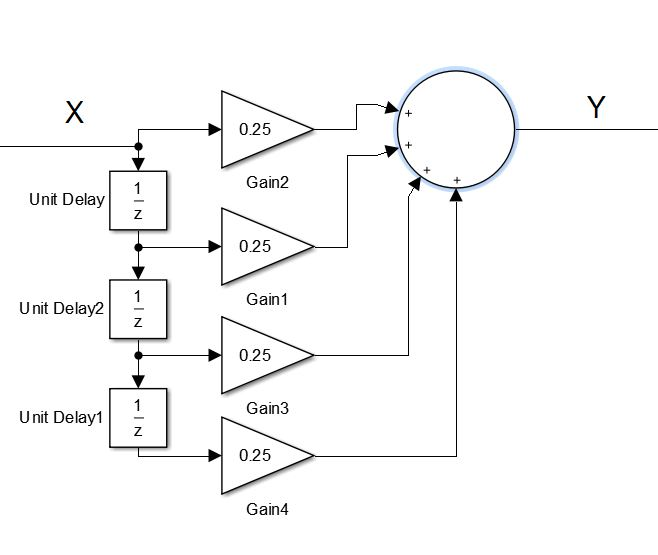
\includegraphics[width=0.8\linewidth]{marius/FIR}
	\caption{Struckturplan FIR}
	\label{fig:FIR}
\end{figure}

\section{Simulationsergebnisse}
\begin{figure}[ht]
	\centering
	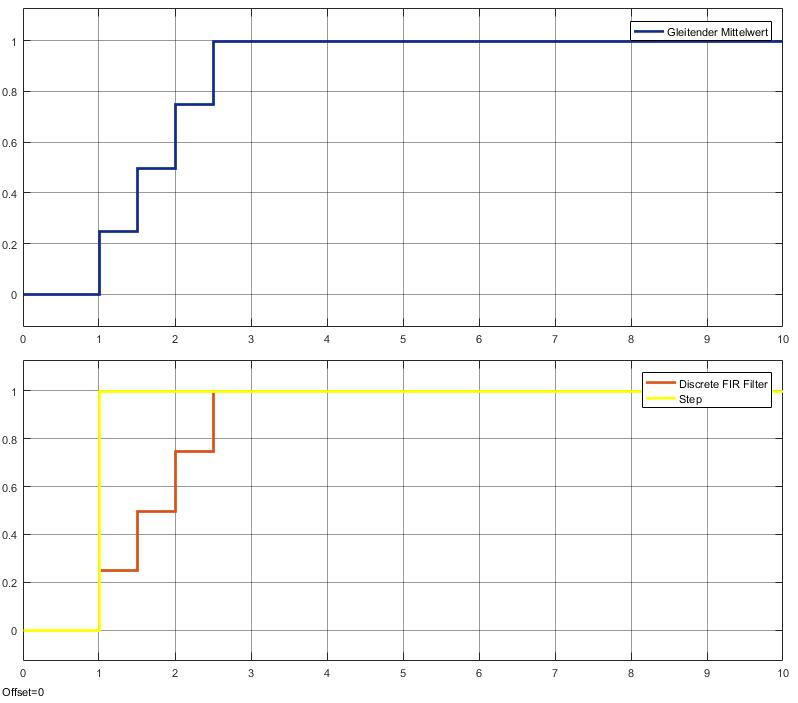
\includegraphics[width=0.9\linewidth]{marius/FIR_Step}
	\caption{Sprungantwort des diskreten FIR-Filters}
	\label{fig:FIR_Step}
\end{figure}
\begin{figure}[ht]
	\centering
	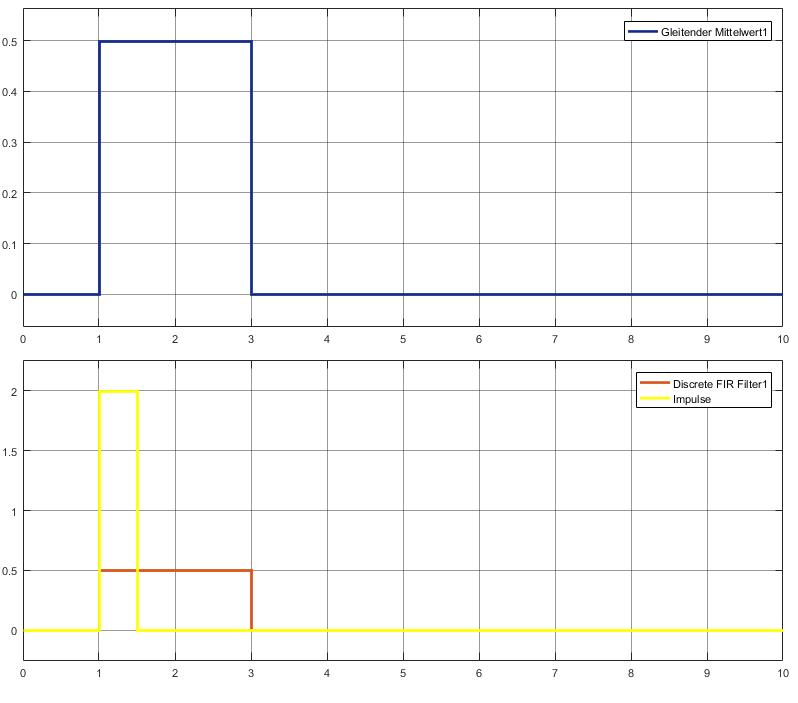
\includegraphics[width=0.9\linewidth]{marius/FIR_Impulse}
	\caption{Impulseantwort des diskreten FIR-Filters}
	\label{fig:FIR_Impulse}
\end{figure}




\end{document}